\begin{tikzpicture}[thick, scale=0.7]
	
	\tikzstyle{partition}=[dashed, very thick]
	\tikzstyle{border}=[help lines, rounded corners]
	
	\tikzstyle{arrow base}=[ gray, fill
	                       , single arrow
	                       , minimum height=0.7*1cm
	                       , minimum width=0.7*1cm
	                       ]
	\tikzstyle{rarrow}=[arrow base, anchor=west]
	\tikzstyle{larrow}=[arrow base, shape border rotate=180, anchor=east]
	\tikzstyle{uarrow}=[arrow base, shape border rotate=90, anchor=south]
	\tikzstyle{darrow}=[arrow base, shape border rotate=270, anchor=north]
	
	% #1 location
	% #2 name
	\newcommand{\process}[2]{
		\node [draw, circle, inner sep=0, minimum width=0.7*1.3em, font=\tiny]
		      (process #2) at (#1)
		      {#2};
	}
	
	% #1 location
	% #2 name
	\newcommand{\cpu}[2]{
		\node [ draw, rectangle, inner sep=0
		      , minimum width=0.7*4em,
		      , minimum height=0.7*4em
		      , font=\footnotesize
		      ]
		      (cpu #2) at (#1)
		      {#2};
	}
	
	% The communication graph
	\process{0, 0}{1}
	\process{1, 1}{2}
	\process{1, -1}{3}
	\process{3, 1}{4}
	\process{3, -1}{5}
	\process{4, -1}{6}
	\draw (process 1) -- (process 2);
	\draw (process 1) -- (process 3);
	\draw (process 2) -- (process 3);
	\draw (process 2) -- (process 4);
	\draw (process 3) -- (process 5);
	\draw (process 4) -- (process 5);
	\draw (process 5) -- (process 6);
	\draw [partition] (2, 1.5) -- (2, -1.5);
	
	% The connection graph
	\begin{scope}[shift={(0.5, -4)}]
		\cpu{0, 0}{a}
		\cpu{3, 0}{b}
		\cpu{0, -3}{c}
		\cpu{3, -3}{d}
		\draw (cpu a) -- (cpu b);
		\draw (cpu b) -- (cpu d);
		\draw (cpu c) -- (cpu d);
		\draw (cpu c) -- (cpu a);
		\draw [partition] (1.5, 1.5) -- (1.5, -4.5);
	\end{scope}
	
	% Border
	\draw [border]
	      ([shift={(-1.5,-2)}]cpu c) coordinate (bl) rectangle
	      ([shift={(1,1)}]process 6 |- process 4) coordinate (tr);
	
	% Arrows
	\node [rarrow] at ([xshift=0.25cm]$(bl-|tr)!0.5!(tr)$) {};
	\node [larrow] at ([xshift=-.25cm]$(bl)!0.5!(tr-|bl)$) {};
	
	% Key
	%\node at ([yshift=6cm]$(tr)!0.5!(tr-|bl)$)
	\node at ([yshift=-1cm]$(bl)!0.5!(tr|-bl)$)
	      (key)
	      {\textbf{Key:}};
	\node [below=0 of key]
	{
		\begin{tikzpicture}[thick, scale=0.7]
			\node [below=0 of key] (partition) {Partition};
			\node at (partition.south west) [anchor=north west] (process) {Process};
			\node at (process.south west) [anchor=north west] (node) {Node};
			
			\draw [partition]
			       ([xshift=-.5em-0.7em]partition.west)
			      +(-0.7em, -0.7em) --
			      +(0.7em, 0.7em);
			\node [left=0.5em of process, draw, circle, minimum width=0.7em, inner sep=0] {};
			\node [left=0.5em of node, draw, rectangle, minimum width=0.7em, minimum height=0.7em, inner sep=0] {};
		\end{tikzpicture}
	};
	
	% Resulting placement
	\node at ([yshift=-5.25cm]$(bl)!0.5!(tr|-bl)$)
	      (placement)
	      {\textbf{Resulting Placement:}};
	\node [below=0 of placement]
	{
		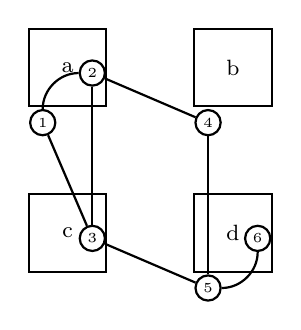
\begin{tikzpicture}[thick, scale=0.7]
			\cpu{0, 0}{a}
			\cpu{3, 0}{b}
			\cpu{0, -3}{c}
			\cpu{3, -3}{d}
			%\draw (cpu a) -- (cpu b);
			%\draw (cpu b) -- (cpu d);
			%\draw (cpu c) -- (cpu d);
			%\draw (cpu c) -- (cpu a);
			
			\process{-0.45, -1}{1}
			\process{0.45, -0.1}{2}
			
			\process{2.55, -1}{4}
			
			\process{0.45, -3.1}{3}
			
			\process{3.45, -3.1}{6}
			\process{2.55, -4}{5}
			
			\draw (process 1)
			      .. controls +(0, 0.6) and +(-0.6, 0) ..
			      (process 2);
			\draw (process 1) -- (process 3);
			\draw (process 2) -- (process 3);
			\draw (process 2) -- (process 4);
			\draw (process 3) -- (process 5);
			\draw (process 4) -- (process 5);
			\draw (process 5)
			      .. controls +(0.6, 0) and +(0, -0.6) ..
			      (process 6);
		\end{tikzpicture}
	};
	
	% Left split of partitions
	\begin{scope}[shift={(-5, -0.25)}]
		\process{0, 0}{1}
		\process{1, 1}{2}
		\process{1, -1}{3}
		\draw (process 1) -- (process 2);
		\draw (process 1) -- (process 3);
		\draw (process 2) -- (process 3);
		\draw [partition] (0, -1) -- (1.5, 0);
		
		\begin{scope}[shift={(0.5, -4)}]
			\cpu{0, 0}{a}
			\cpu{0, -3}{c}
			\draw (cpu c) -- (cpu a);
			\draw [partition] (-1.5, -1.5) -- (1.5, -1.5);
		\end{scope}
		
		% Border
		\draw [border]
		      ([shift={(-2,-1.5)}]cpu c) coordinate (bl) rectangle
		      ([shift={(1.5,1)}]process 2) coordinate (tr);
		
		% Arrows
		\node [uarrow] at ([yshift=0.25cm]$(bl|-tr)!0.5!(tr)$) {};
		\node [darrow] at ([yshift=-.25cm]$(bl)!0.5!(bl-|tr)$) {};
		
		% Top sub-split
		\begin{scope}[shift={(0, 7)}]
			\process{0, 0}{1}
			\process{1, 1}{2}
			\draw (process 1) -- (process 2);
			
			\begin{scope}[shift={(0.5, -2)}]
				\cpu{0, 0}{a}
			\end{scope}
			
			% Border
			\draw [border]
			      ([shift={(-1.5,-1.5)}]cpu a) rectangle
			      ([shift={(1,1)}]process 2);
		\end{scope}
		
		% Bottom sub-split
		\begin{scope}[shift={(0, -11)}]
			\process{0.5, 0}{3}
			
			\begin{scope}[shift={(0.5, -2)}]
				\cpu{0, 0}{c}
			\end{scope}
			
			% Border
			\draw [border]
			      ([shift={(-1.5,-1.5)}]cpu c) rectangle
			      ([shift={(1.5,1)}]process 3);
		\end{scope}
	\end{scope}
	
	% Right split of partitions
	\begin{scope}[shift={(8, -0.25)}]
		\process{0, 1}{4}
		\process{0, -1}{5}
		\process{1, -1}{6}
		\draw (process 4) -- (process 5);
		\draw (process 5) -- (process 6);
		\draw [partition] (-0.5, 0) -- (0.5, 0);
		
		\begin{scope}[shift={(0.5, -4)}]
			\cpu{0, 0}{b}
			\cpu{0, -3}{d}
			\draw (cpu b) -- (cpu d);
			\draw [partition] (-1.5, -1.5) -- (1.5, -1.5);
		\end{scope}
		
		% Border
		\draw [border]
		      ([shift={(-2,-1.5)}]cpu d) coordinate (bl) rectangle
		      ([shift={(1.5,1)}]process 6 |- process 4) coordinate (tr);
		
		% Arrows
		\node [uarrow] at ([yshift=0.25cm]$(bl|-tr)!0.5!(tr)$) {};
		\node [darrow] at ([yshift=-.25cm]$(bl)!0.5!(bl-|tr)$) {};
		
		% Top sub-split
		\begin{scope}[shift={(0, 7)}]
			\process{0.5, 0}{4}
			
			\begin{scope}[shift={(0.5, -2)}]
				\cpu{0, 0}{b}
			\end{scope}
			
			% Border
			\draw [border]
			      ([shift={(-1.5,-1.5)}]cpu b) rectangle
			      ([shift={(1.5,1)}]process 4);
		\end{scope}
		
		% Bottom sub-split
		\begin{scope}[shift={(0, -11)}]
			\process{0, 0}{5}
			\process{1, 0}{6}
			\draw (process 5) -- (process 6);
			
			\begin{scope}[shift={(0.5, -2)}]
				\cpu{0, 0}{d}
			\end{scope}
			
			% Border
			\draw [border]
			      ([shift={(-1.5,-1.5)}]cpu d) rectangle
			      ([shift={(1,1)}]process 6);
		\end{scope}
	\end{scope}
	
\end{tikzpicture}
